\section{Requirements specification for Administration Module}\label{Administration components}

\subsection{General Definition}\label{General Definition AMC}

Administration Module Component (AMC) is an application, which is responsible for managing OpenStack and Cloudify. It embeds the Monitoring System and Alert Management System. AMC is integrated into N2Sky cloud platform in order to support the N2Sky environment and services. This component is implementing Platform as a Service approach, hence it can be installed on any cloud server. 

\subsection{Affected Users}\label{Affected users}

The users, who have full knowledge about the domain with corespondent permissions or domain owner, can have an access to AMC.

In N2Sky, only System Administrator has a proper main function in order to manage AMC.
Following functions are available for System Administrator:
\begin{itemize}
\item Mange own dashboard
\item Control OpenStack dashboard and its services
\item Control Cloudify dashboard and its services
\item Manage monitoring charts
\item Manage alerts and alerting rules
\item Manage the OpenStack instances (servers)
\item Has an access to dashboards of other users
\end{itemize}



\subsection{Administration Dashboard}\label{Administration Dashboard}

Administration Dashboard represents the overview of administration tools and important metrics, which are displayed in figure ~\ref{fig:admin_dashboard}. 

\begin{figure}[htbp]
\begin{center}
  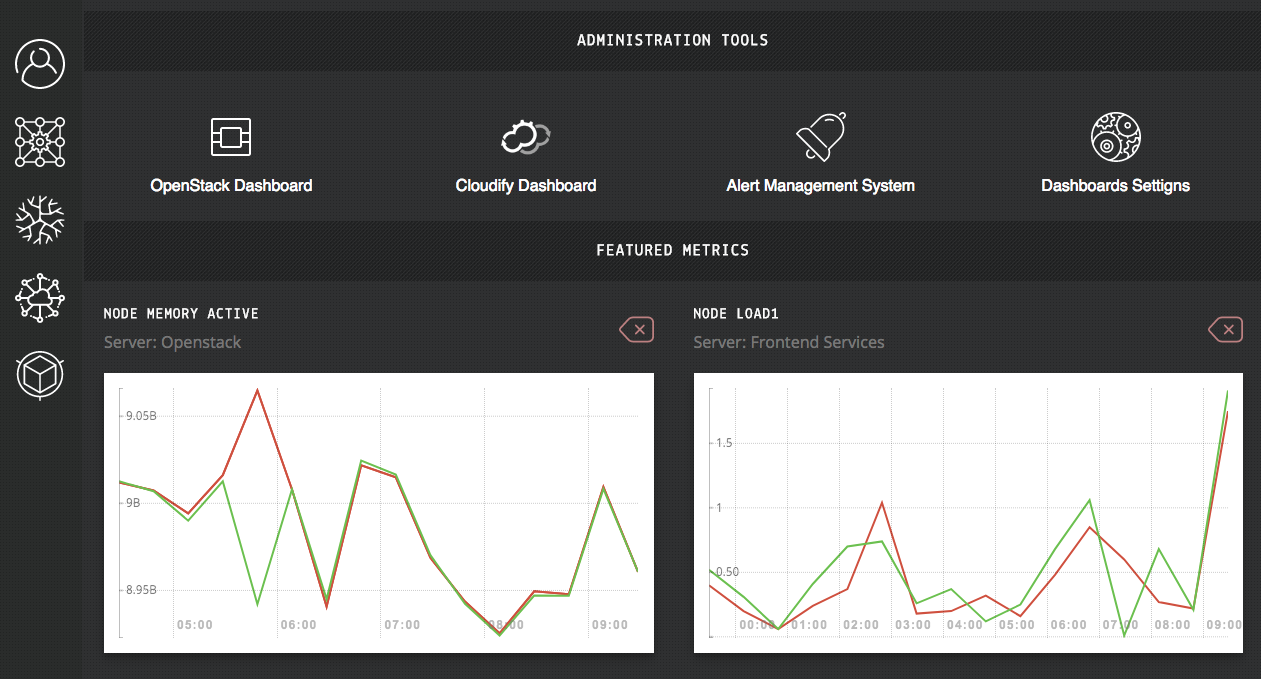
\includegraphics[width=\linewidth]{components/4/pics/admin_dashboard.png}
  \caption{N2Sky Administration Dashboard.}
  \label{fig:admin_dashboard}
\end{center}
\end{figure}

After System Administrator authorise in the system, he will be automatically redirected to the Administration Dashboard. By default, URL link is:
\begin{lstlisting}
        <host>/cloud
\end{lstlisting}

Administration tools have to be in focus of the main dashboard view as shown in figure \ref{fig:admin_tools}. The collection of elements has to be under the title bar element, which is named "ADMINISTRATION TOOLS". Every element of administration tool contains an icon in SVG \cite{Cagle2005} format and caption under it. Following administration tools have to be represented: 
\begin{itemize}
\item OpenStack Dashboard. Link to view: 
\begin{lstlisting}
        <host>/openstack
\end{lstlisting}
\item Cloudify Dashboard. Link to view: 
\begin{lstlisting}
        <host>/cloudify
\end{lstlisting}
\item Alert Management System. Link to view: 
\begin{lstlisting}
        <host>/alert
\end{lstlisting}
\item Dashboards Settings. Modal popup window without redirection
\end{itemize}

\begin{figure}[H]
\begin{center}
  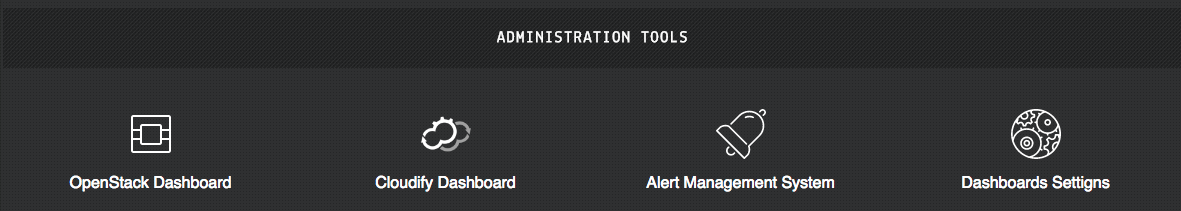
\includegraphics[width=\linewidth]{components/4/pics/admin_tools.png}
  \caption{N2Sky Administration Dashboard. Administration tools component.}
  \label{fig:admin_tools}
\end{center}
\end{figure}

Next to the administration tools, the monitoring charts are visible. The title of this block is "FEATURED METRICS", which is the title bar upon the metrics.
Every chart is a grid item element and the grid itself has to contain a maximum of two grid items in one row as shown in figure \ref{fig:featured_metrics}. 
 
\begin{figure}[H]
\begin{center}
  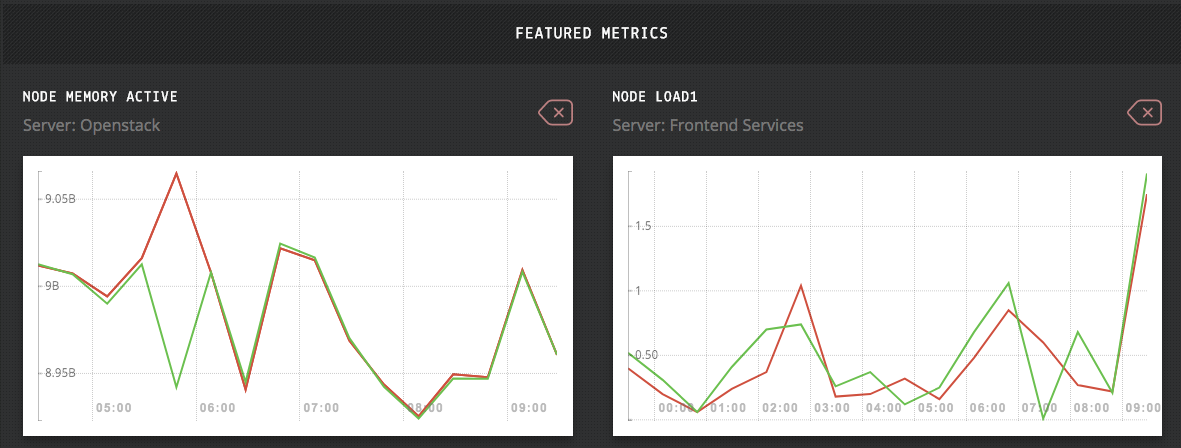
\includegraphics[width=\linewidth]{components/4/pics/featured_metrics.png}
  \caption{N2Sky Administration Dashboard. Featured Metrics component.}
  \label{fig:featured_metrics}
\end{center}
\end{figure}
 
 
The user decides by himself which monitoring charts will be shown. The configuration is located in "Dashboard Settings" administration tool element. More details about the creation of monitoring charts are located in \autoref{Monitoring System}. 


\subsection{Openstack Dashboard}\label{OpenStack Dashboard}

OpenStack Dashboard is the dashboard for managing OpenStack and its services. It also displays the monitoring of OpenStack and its instances. It looks similar to the Administration Dashboard, except that it is the only oriented OpenStack and there are no additional tools as shown in figure \ref{fig:openstack_dashboard}. 

\begin{figure}[H]
\begin{center}
  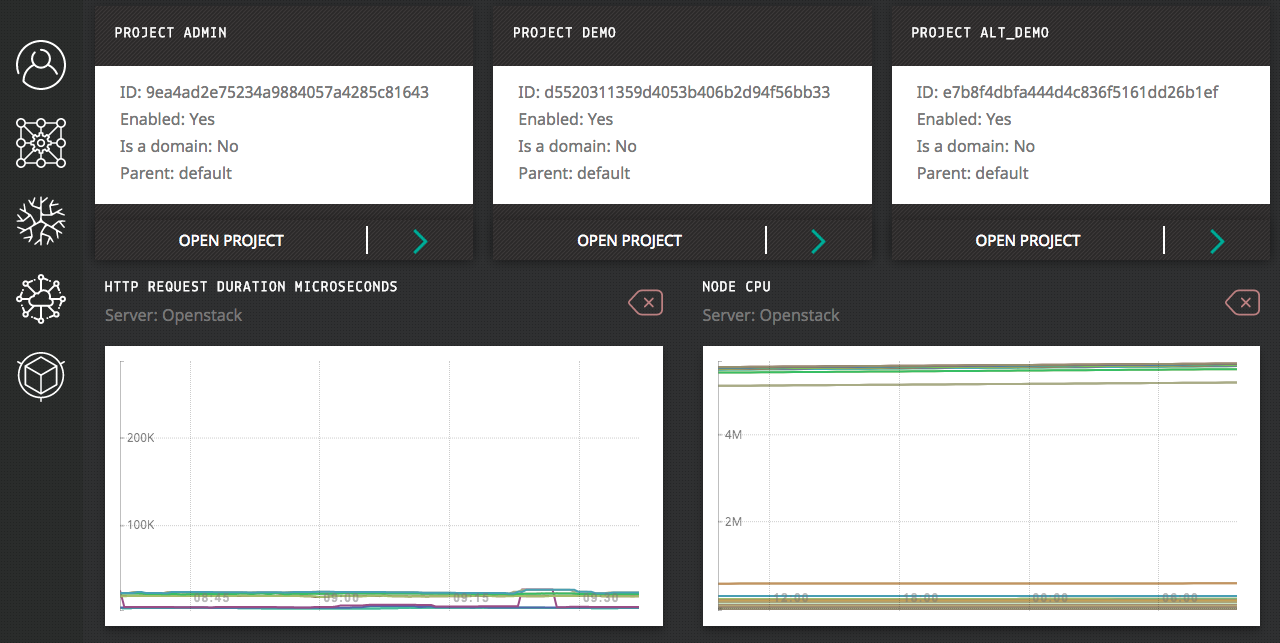
\includegraphics[width=\linewidth]{components/4/pics/openstack_dashboard.png}
  \caption{N2Sky OpenStack Dashboard.}
  \label{fig:openstack_dashboard}
\end{center}
\end{figure}
 

This dashboard contains two blocks:

\begin{description}
\item[Project grid.] This block contains projects, which are available on OpenStack as shown in figure \ref{fig:openstack_dashboard_projects}.

\begin{figure}[H]
\begin{center}
  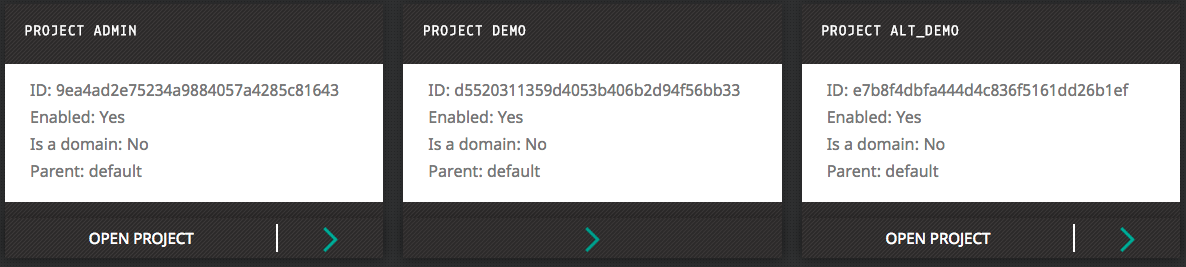
\includegraphics[width=\linewidth]{components/4/pics/openstack_dashboard_projects.png}
  \caption{N2Sky OpenStack Dashboard. Projects grid}
  \label{fig:openstack_dashboard_projects}
\end{center}
\end{figure}

Every grid item represents a brief overview of the OpenStack Project:

\begin{itemize}
\item Name of the project, which is the header of the grid item.
\item ID of the project.
\item Enabled, which stays if available (value YES) or not available (value NO).
\item Is a domain, also contains simple yes or no values.
\item Parent, which shows if there any parent project which the current project is linked to.
\item Button "Open Project", which redirects to the project details.
\end{itemize}

\item[Monitoring Grid.] Similar to the Administration Dashboard, the monitoring grid can be customized by users. Detailed information about customization is written in \autoref{Monitoring System}. 

\end{description}

After being redirected to the project details, the user will see the information about the specific project. Redirection should have the following URL path: 
\begin{lstlisting}
        <host>/openstack/project/<id>
\end{lstlisting}

Where <id> is the OpenStack project ID.

\subsubsection{OpenStack Nova Service}\label{OpenStack Nova Service}

Nova is a compute service of OpenStack. It gives an overview and manages all existing virtual machines (servers or instances) \cite{Markelov2016}. 

Following tools are used by this compute service:
\begin{itemize}
\item Horizon. Web UI for managing OpenStack projects. It is not used in the N2Sky system since N2Sky Web UI has its own interface for managing the OpenStack instances.
\item OpenStack Client, which includes commands for Nova as well as for OpenStack projects.
\item Nova Client, which can be used like OpenStack Client. N2Sky does not use it since OpenStack Client can provide all needed commands for nova service. 
\end{itemize}


The OpenStack project view has detailed description about the server and its instances as shown in figure \ref{fig:openstack_project_view}. 

\begin{figure}[H]
\begin{center}
  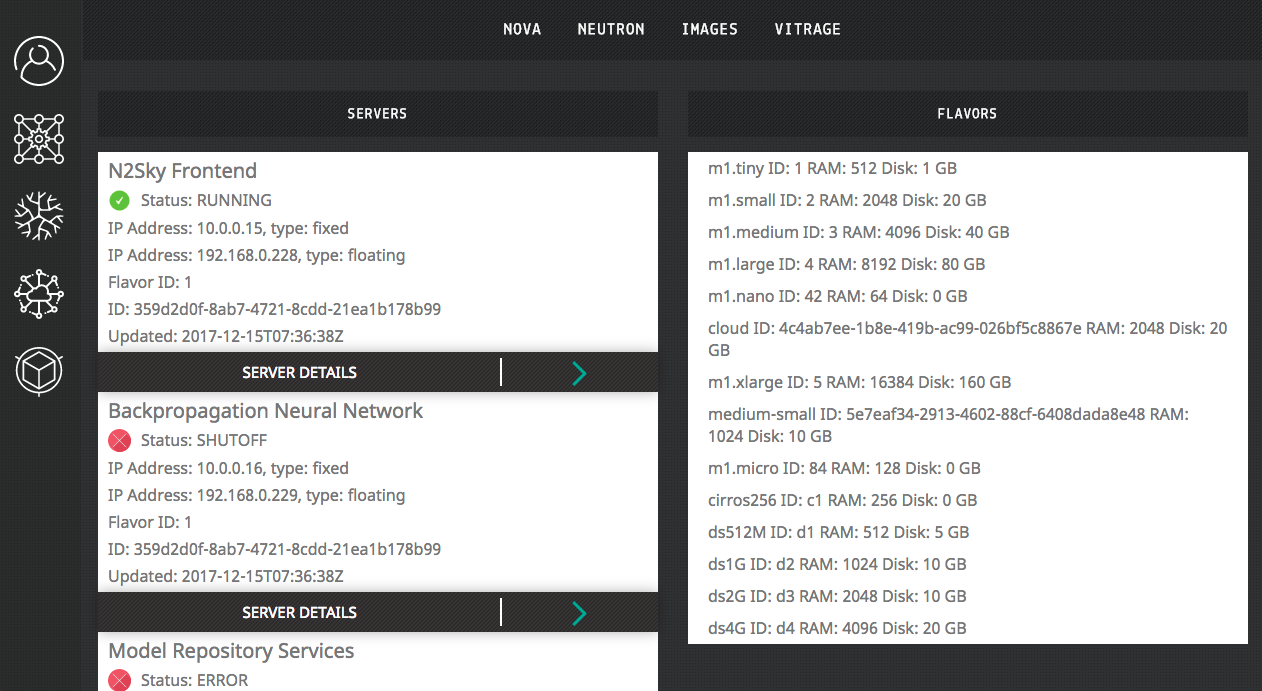
\includegraphics[width=\linewidth]{components/4/pics/openstack_project_view.png}
  \caption{N2Sky OpenStack Dashboard. Project view}
  \label{fig:openstack_project_view}
\end{center}
\end{figure}

This view contains following components:
\begin{description}
\item[Navigation Bar.] Navigation over OpenStack Services namely:
\begin{itemize}
\item NOVA
\item NEUTRON
\item IMAGES
\item VITRAGE
\end{itemize}
 
 \item[Servers.] The servers item grid is located on the left side of the screen and has a collection of servers (OpenStack instances) as shown in figure \ref{fig:openstack_servers}. 
 
 \begin{figure}[H]
\begin{center}
  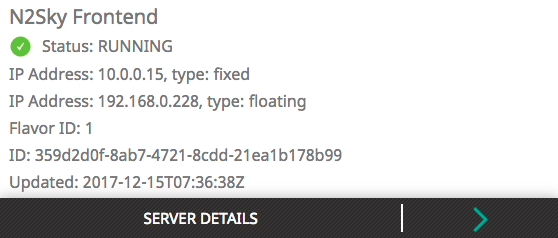
\includegraphics[scale=0.5]{components/4/pics/openstack_servers.png}
  \caption{N2Sky OpenStack Dashboard. Server overview}
  \label{fig:openstack_servers}
\end{center}
\end{figure}

The server overview grid contains following elements:
\begin{itemize}
\item Server name 
\item Status, which can be: 
\begin{itemize}
\item RUNNING - instance is running and available. 
\item SHUTOFF - instance is shut down manually or by scheduler. 
\item ERROR - an error occurs during spawning an instance or the instance went down during the run.
\end{itemize}
\item IP Address fixed. The IP Address for instance inside OpenStack Cloud.
\item IP Address floating. Assigned to instance IP address. Through this IP address, external access to the instance is possible. 
\item Flavor ID. Reference to OpenStack flavor, which is located on the right side of OpenStack project view.
\item ID of the server (OpenStack instance).
\item Updated is a timestamp when the instance was for the last time modified. 
\end{itemize}
\item[Flavors.] A flavor is defined as an environment configuration. In the project details view, there is the list of flavors. On click on the particular flavor of this list, the flavor details will appear as shown in figure \ref{fig:openstack_flavors}.

 \begin{figure}[htbp]
\begin{center}
  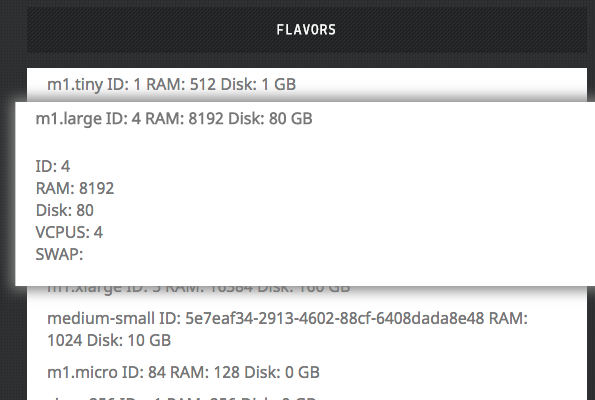
\includegraphics[scale=0.5]{components/4/pics/openstack_flavors.png}
  \caption{N2Sky OpenStack Dashboard. Flavors}
  \label{fig:openstack_flavors}
\end{center}
\end{figure}

Following elements are displayed: 
\begin{itemize}
\item Type of flavor, which is defined by OpenStack.
\item ID of flavor. OpenStack instances have a reference to particular flavor ID
\item RAM. Amount of available memory of particular flavor. 
\item Disk space in GB, which is available for a particular flavor. 
\item VCPUS. About of CPUs which will be available. 
\item SWAP in GB, which is set for the particular flavor.
\end{itemize}

\end{description}

When the user chooses some server (instance), he will be redirected to the server details view as shown in figure \ref{fig:openstack_server_details}.

 \begin{figure}[H]
\begin{center}
  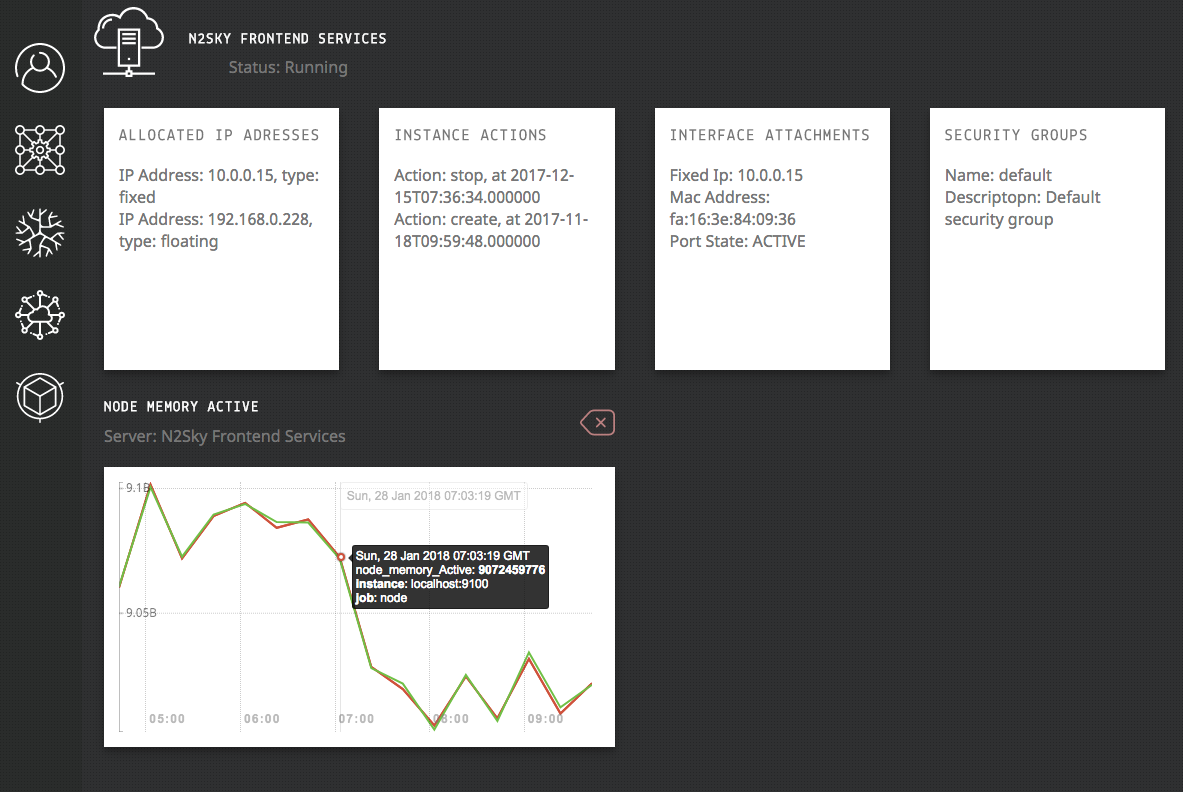
\includegraphics[width=\linewidth]{components/4/pics/openstack_server_details.png}
  \caption{N2Sky OpenStack Dashboard. Server details view.}
  \label{fig:openstack_server_details}
\end{center}
\end{figure}

\subsubsection{OpenStack Neutron Service}\label{OpenStack Neutron Service}

Neutron is an OpenStack networking service, which provides "network connectivity as a service". Neutron is fully integrated into the OpenStack UI, which allows managing networking directly from there. The networking service is based on quantum architecture, where API clients communicate with virtual switches through Quantum API and Quantum plugin \cite{neutron}. This service implements Neutron API, which is used by the N2Sky Web UI. 

Neutron Service is integrated into N2Sky and represents the overview of networks, subnet pools, and services providers as shown in figure \ref{fig:openstack_neutron}.

\begin{figure}[H]
\begin{center}
  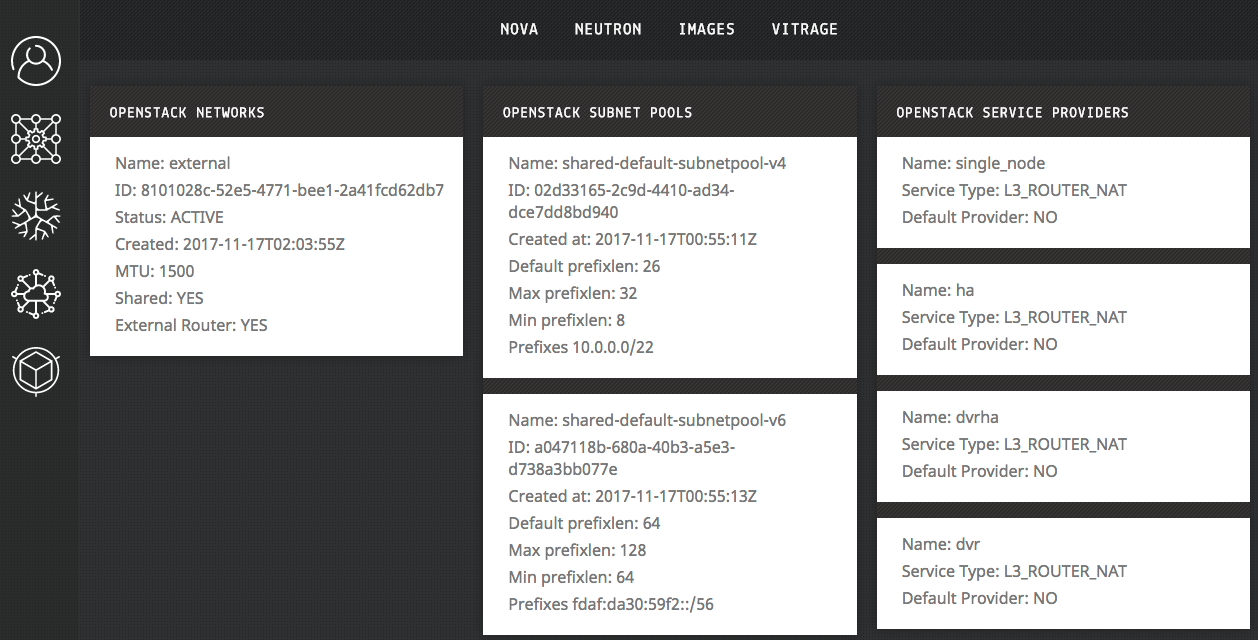
\includegraphics[width=\linewidth]{components/4/pics/openstack_neutron.png}
  \caption{N2Sky OpenStack Dashboard. Neutron Service View}
  \label{fig:openstack_neutron}
\end{center}
\end{figure}

The server details view contains following components:
\begin{description}
\item[Header.] Header of this view contains the name of the server, icon, and status, which can be "Running" if the instance is available and running on OpenStack environment, "Shutdown" if the instance is available but not running or an "Error" in case of an error occurring. 
\item[Instance information grid]. The following grid represents summary information about the server (instance) and consist of these items:
\begin{itemize}
\item Allocated IP Address is a list of assigned to instance IP addresses. Every IP address has a type either "fixed" or "floating".
\item Instance actions is a list of all activities and events, which happened in the particular instance. Log information contains the action type and timestamp of action.
\item Interface attachments, which contains fixed IP address, mac address add port state ("ACTIVE" or "INACTIVE") of the instance.
\item Security groups is a list of security groups which contains the name and description of the security group. 
\end{itemize}
\item[Monitoring.] The grid of monitoring charts of the particular server. Can be removed directly from the view or added via the navigation menu or Administration Dashboard.
\end{description}


The grid represents following components besides the navigation bar: 
\begin{description}
\item[OpenStack Networks.]  The list of available networks on OpenStack cloud. Every network contains the following information:
\begin{enumerate}
\item Name of the network
\item ID of the network
\item Status, which can be "ACTIVE" if the network is available and "INACTIVE" if not available or an error occurred. 
\item Created is the timestamp of creation of the network
\item MTU (Network Service Uses), which are based on a physical network in order to calculate the MTU of the virtual network components. 
\item Shared. "YES" for shared access and "NO" for not shared. 
\item External router. "YES" if an external router is attached and "NO" for not attached. 
\end{enumerate}
\item[OpenStack Subnet Pools.] This service provides information about available subnetworks and includes following information on the N2Sky application:
\begin{enumerate}
\item Name of the subnetwork
\item ID of the subnetwork
\item Created at is the timestamp of subnetwork creation
\item Default number prefixlen
\item Max number of prefixlen
\item Min number of prefixlen
\item Prefixlen, which represents a pool prefix
\end{enumerate}
\item[OpenStack Service Providers.] The list of created and available service providers with customized configuration, which contains:
\begin{enumerate}
\item Name of service provider
\item Service type
\item Default Provider. "YES" if it exists, "NO" if not.  
\end{enumerate}

\end{description}


\subsubsection{OpenStack Images Service}\label{OpenStack Images Service}

In OpenStack is possible to upload customized images of the Virtual Machine to the provider. N2Sky uses the Images Service only for the representation of images information. The user can download an image, but it is not possible to upload customized image due to the expensive process, because of the image size. It is possible to use template provider with pre-configured virtual machine \cite{images}. 


\begin{figure}[H]
\begin{center}
  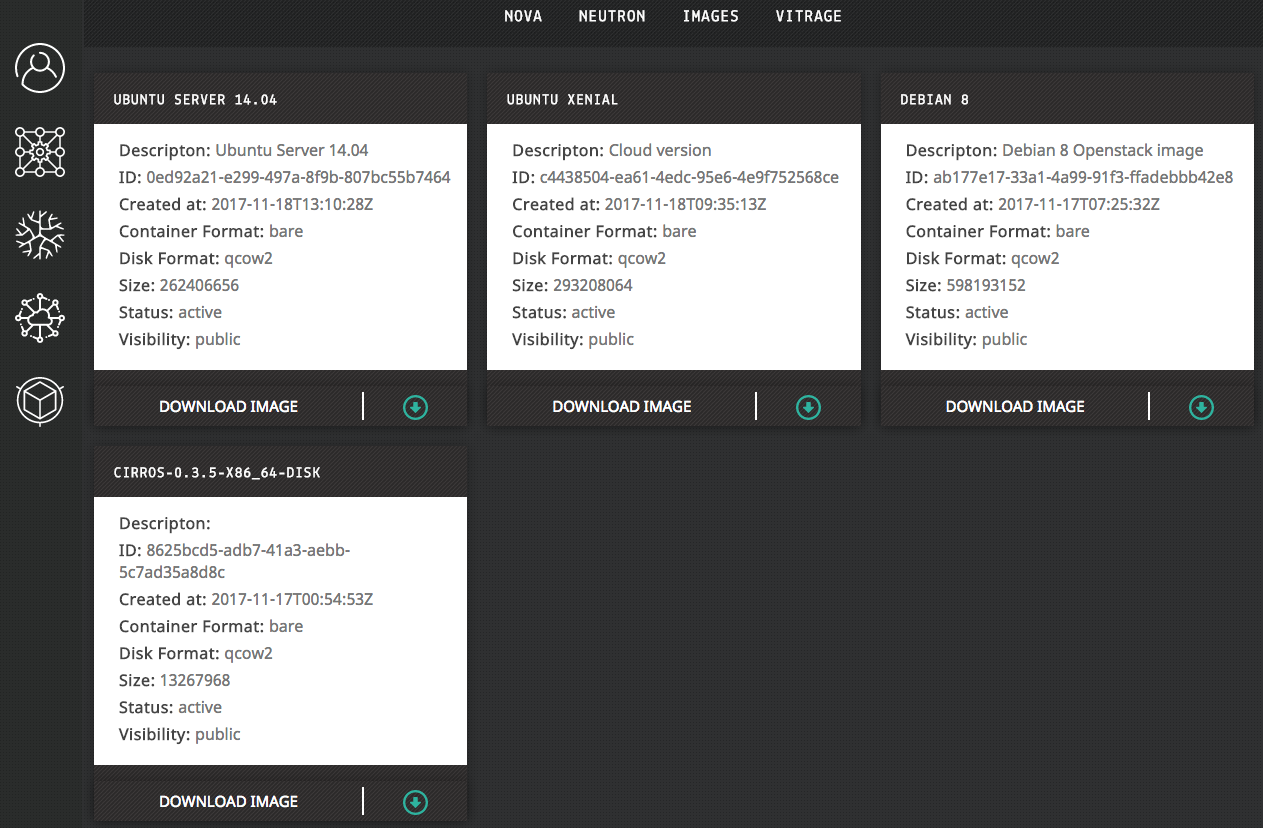
\includegraphics[width=\linewidth]{components/4/pics/openstack_images.png}
  \caption{N2Sky OpenStack Dashboard. Images Service View}
  \label{fig:openstack_images}
\end{center}
\end{figure}

The Image Service view, shown in figure \ref{fig:openstack_images} is representing a grid of available images. Every grid item contains the following information: 
\begin{enumerate}
\item Name of the image
\item Description of the image
\item ID of the image
\item Created at, which represents the timestamp of the creation date of the image
\item Container format
\item Disk format, namely format of the image (qcow2 is a typical format for OpenStack instance)
\item Size of the image in bytes
\item Status of the image. Active if image is successfully uploaded and ready to use, inactive if not
\item Visibility. Public for everyone, or group name for a particular group of OpenStack users
\item Download image button, which creates one more thread and initializes the downloading procedure
\end{enumerate}

There are custom OpenStack image templates and configurations created for the N2Sky system. Every image has to contain the following configuration:
\begin{itemize}
\item Preinstalled Docker CLI
\item N2Sky Monitoring System instance
\item N2Sky Alert Management System rules configuration
\end{itemize}

N2Sky templates and configuration have to support the following operating systems:
\begin{itemize}
\item Ubuntu 14.04 / 16.04 
\item Debian 8
\item Centos
\end{itemize}



\subsubsection{OpenStack Vitrage Service}\label{OpenStack Vitrage Service}

Vitrage is the OpenStack RCA (Root Cause Analysis) service. It is build in the monitoring system, which helps to analyze and organize the OpenStack alarms and events \cite{wiki:vitrage}. In the N2Sky platform, the Vitrage service is used only for representation of templates and resources because N2Sky has its own Monitoring System, which can be propagated in all OpenStack instances.  

\begin{figure}[H]
\begin{center}
  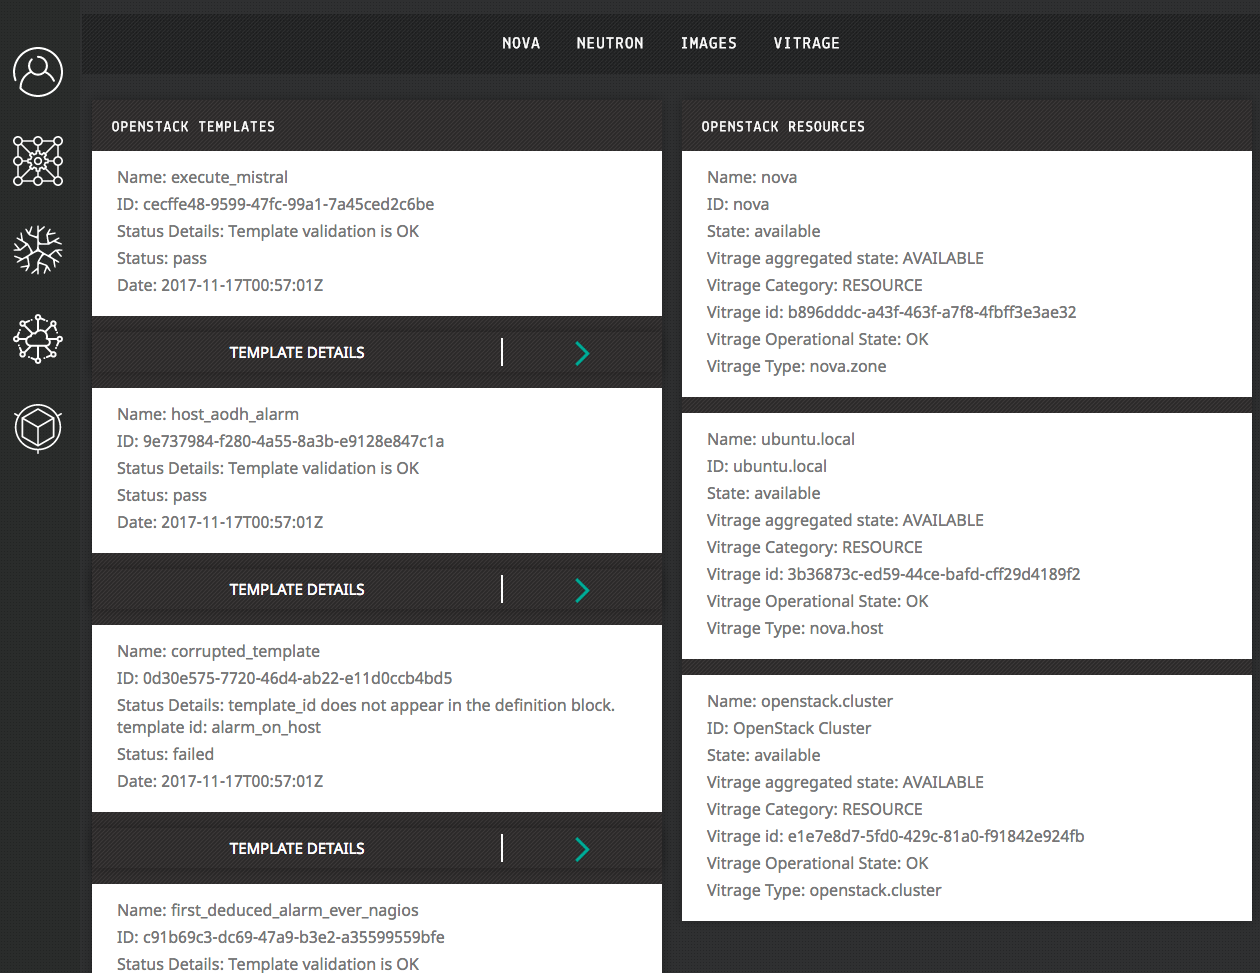
\includegraphics[width=\linewidth]{components/4/pics/opentack_vitrage.png}
  \caption{N2Sky OpenStack Dashboard. Vitrage Service View}
  \label{fig:opentack_vitrage}
\end{center}
\end{figure}

The two column grid view shown in figure \ref{fig:opentack_vitrage}, represents the following grid items:

\begin{description}
\item[OpenStack Templates.]  List of OpenStack templates with following data:
\begin{enumerate}
\item Name of the template
\item ID of the template
\item Status Details, which shows if the template is validated 
\item Date, which shows the timestamp of template creation 
\item Template details button, which redirects in detailed information about the chosen template
\end{enumerate}

\item[OpenStack Resources.] List of available OpenStack resources, which contains following data:
\begin{enumerate}
\item Name of the resource
\item ID of the resource
\item State of the resource can be available or not
\item Vitrage aggregated state can be available or not
\item Vitrage Category can be resource, alarm or another customized category
\item Vitrage ID
\item Vitrage Operational State
\item Vitrage Type
\end{enumerate}
\end{description}

\begin{figure}[htbp]
\begin{center}
  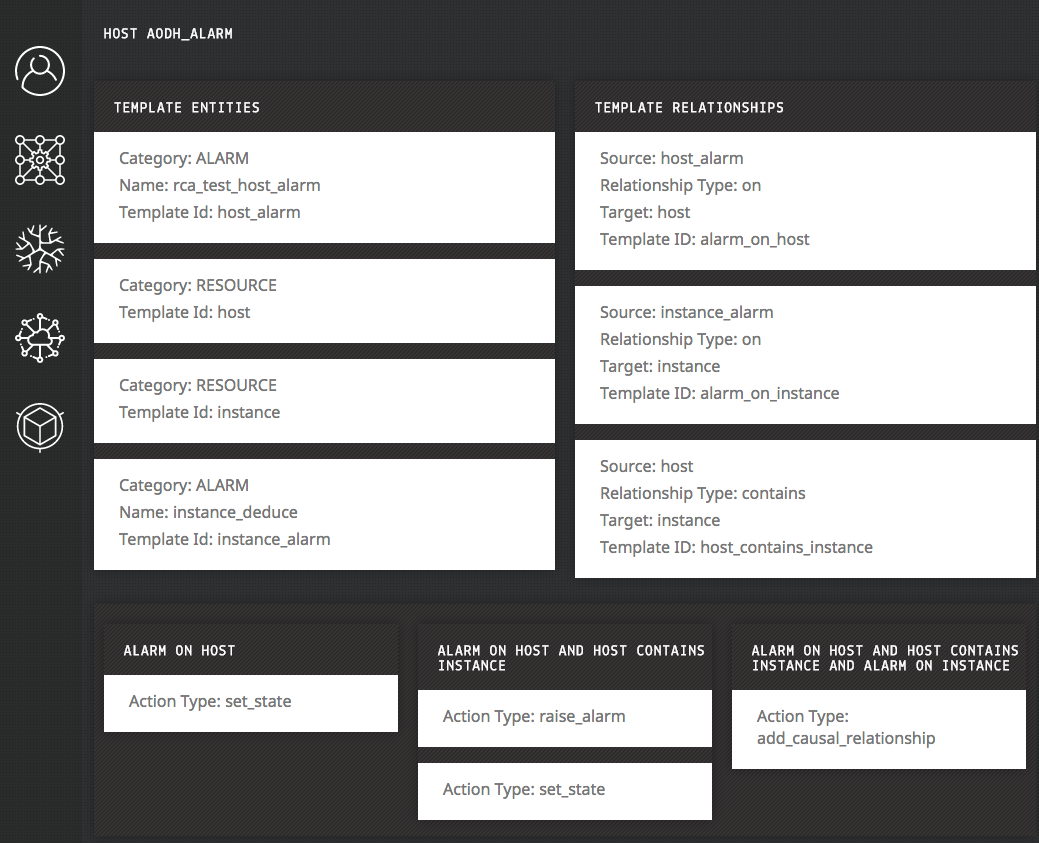
\includegraphics[width=\linewidth]{components/4/pics/openstack_template.png}
  \caption{N2Sky OpenStack Dashboard. Template Details View}
  \label{fig:openstack_template}
\end{center}
\end{figure}

When the user clicks on the template details button, he will be redirected to a particular Vitrage template as shown in figure \ref{fig:openstack_template}. From here, the user can observe the following information:
\begin{description}
\item[Template Entities]. List of entities like alarm or resource. This grid item contains the following data:
\begin{enumerate}
\item Template ID (mandatory)
\item Name of the template (optional)
\item Template category (optional)
\end{enumerate}
\item[Template Relationships]. List of relationships between templates, which reference from source to target.
\begin{enumerate}
\item Source entity
\item Target entity
\item Relationship type
\item Template ID
\end{enumerate}
\item[Alarm On Host.] The action type of the alarm
\item[Alarm on host and host contains instance.] Optional item, visible only if host contains instance.
\item[Alarm on host and host contains instance an alarm on the instance.] Optional item, visible only if host contains instance and alarm on the instance.

\end{description}



%\subsection{Cloudify Dashboard}\label{Cloudify Dashboard}

%\hl{TODO ????}

\subsection{Dashboard Settings}\label{Dashboard Settings}
As it was mentioned before, in the Administration Dashboard chapter \autoref{Administration Dashboard}, the dashboard contains the administration tools. One of these tools is the Dashboard Settings tool. When the user clicks on this tool, the modal popup window will open and available configuration options will appear as shown in figure \ref{fig:openstack_template}.

\begin{figure}[htbp]
\begin{center}
  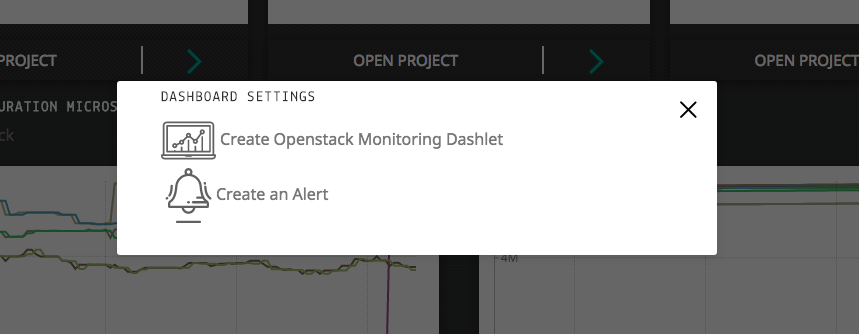
\includegraphics[width=\linewidth]{components/4/pics/dashboard_settings.png}
  \caption{N2Sky Administration Dashboard. Dashboard Settings}
  \label{fig:dashboard_settings}
\end{center}
\end{figure}

Another possibility to initiate the settings popup, is to open it from the main navigation menu, available across the entire application on the left screen of the page view. 

The Dashboard Settings popup contains two settings:
\begin{itemize}
\item Create OpenStack Monitoring Dashlet, which creates one more modal popup upon the existing and initializes the creation of the monitoring chart, described in chapter "Monitoring System" in \autoref{Monitoring System}.
\item Create an Alert, which also creates another modal popup upon the existing and initializes the creation of the alerting rule, described in chapter "Alert System" in \autoref{Alerting System}.
\end{itemize}

The popup will be automatically closed only after the action is performed. If not, the user can leave the popup manually.



\subsection{Monitoring System}\label{Monitoring System}

When Administration Dashboard shows the overview of the OpenStack and Cloudify, the monitoring system goes through every dashboard and applies monitoring charts on user request. There are two main parts, mentioned in FRS: displaying of monitoring charts and management of metrics.
 
\subsubsection{Monitoring Charts Creation}\label{Monitoring charts creation}

After a user initializes the creation of monitoring metrics, described in \autoref{Dashboard Settings} "Dashboard Settings", a new modal window will be opened as shown in figure \ref{fig:create_monitoring}.

\begin{figure}[H]
\begin{center}
  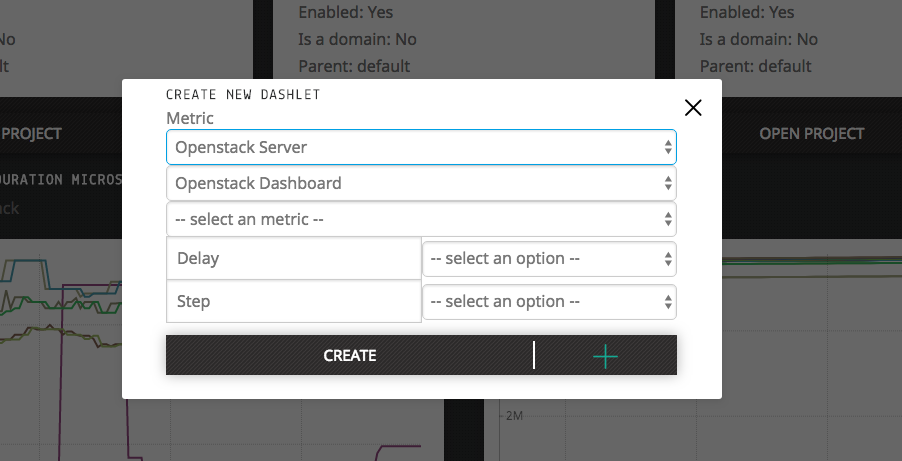
\includegraphics[width=\linewidth]{components/4/pics/create_monitoring.png}
  \caption{N2Sky Administration Dashboard. Monitoring charts creation modal popup}
  \label{fig:create_monitoring}
\end{center}
\end{figure}

The popup window has following elements:

\begin{enumerate}
\item "CREATE NEW DASHLET" title of the popup
\item Combobox with servers, where the monitoring system instance is installed. The user can choose all available instances, even if they are not running currently. It is also possible to choose the OpenStack cloud server itself because the monitoring system instance is preinstalled there.
\item Combobox with views.  The user can choose where the combo box will be added. There are few places where charts can be displayed:
\begin{enumerate}
\item Administration Dashboard
\item OpenStack Dashboard
\item Cloudify Dashboard
\item Servers (OpenStack instances) View. 
\end{enumerate}
\item Combobox with metrics. Normally, there are more than hundreds of available metrics. Every operating system has different naming for metrics.
\item Delay input. This input shows the delayed time of metric.
\item Step input. This input shows the line chart step of chosen metric
\item Timing combo box. This combo box contains following time options:
\begin{enumerate}
\item seconds
\item minutes
\item hours
\item days
\item weeks
\end{enumerate}
\item Create button, which triggers metrics creation. The view will be reloaded and monitoring chart will appear in this view.
\end{enumerate}

After adding a new monitoring chart, the view will be reloaded and the chart will appear on the view. 

\subsubsection{Monitoring Charts Representation}\label{Monitoring chart representation}

Every monitoring chart is a grid item of two column responsive grid as shown in figure \ref{fig:moniroting_representation}

\begin{figure}[htbp]
\begin{center}
  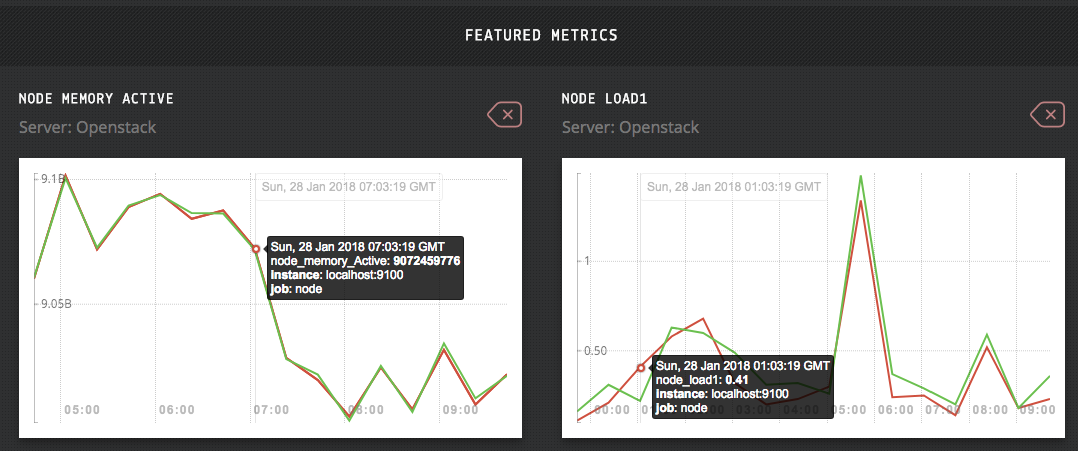
\includegraphics[width=\linewidth]{components/4/pics/moniroting_representation.png}
  \caption{N2Sky Administration Dashboard. Monitoring charts representation}
  \label{fig:moniroting_representation}
\end{center}
\end{figure}

The grid has to be responsive in order to support mobile devices. When the mobile device is detected, the grid should have only one column and its items have to be aligned vertically. 

The header of the monitoring chart has to contain the name of the metrics and the server (instance) from where these metrics come from.

Every monitoring chart has at least one line graph with a random color. If there are a few lines in the graphs chart, then lines should have different colors. Each chart contains on X-axis, the timestamp and on y-Axis, the velocity.  The timestamp, in the line graph, has its own toolkit with additional information about the chart and contains the following data:

\begin{itemize}
\item Timestamp of event
\item Type of metrics and Id of timestamp
\item Instance, where monitoring system is running
\item The name of the job, which is responsible for particular event
\end{itemize}


\subsection{Alert System}\label{Alerting System}

The Alert System has its own page view. It is possible to be redirected to this view from the main navigation menu as well as from the administration dashboard. The URL of the alert page is:
\begin{lstlisting}
        <host>/alert
\end{lstlisting}

\subsubsection{Alerting rule Creation}\label{Alerting rule creation}

Alert rules can be created directly from the alert page view. The button "Create Alert" initiates the modal popup window as shown in figure \ref{fig:alert_create}.

\begin{figure}[H]
\begin{center}
  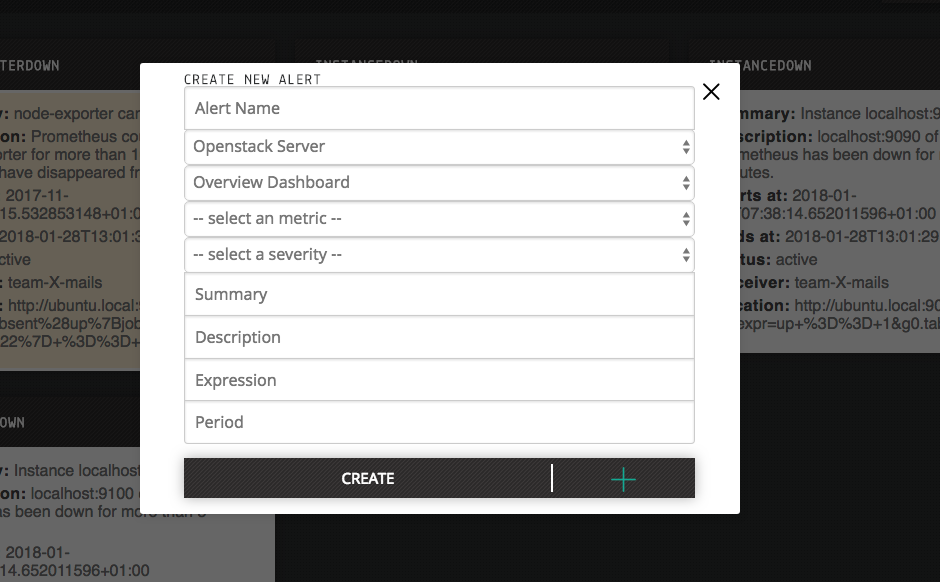
\includegraphics[width=\linewidth]{components/4/pics/alert_create.png}
  \caption{N2Sky Administration Dashboard. Alerting rule creation}
  \label{fig:alert_create}
\end{center}
\end{figure}

The modal window has following elements:
\begin{enumerate}
\item Modal window title is "Create new alert".
\item Combobox with available servers with the installed monitoring system.
\item Combobox with a page view, where an alert can be shown (optional).
\item Combobox with an available metrics.
\item Combobox with alerting rule severity level. Three values are possible: "page", "warning" and "critical".
\item Summary information about alerting rules.
\item Full description of alerting rules.
\item Expression which will be executed against chosen metric.
\item Period, which shows how often will the alerting rule be validated.
\end{enumerate}



\subsubsection{Alerts Representation}\label{Alerts representation}

The alerts are displayed in a three column grid as shown in figure \ref{fig:alert_representation}

\begin{figure}[H]
\begin{center}
  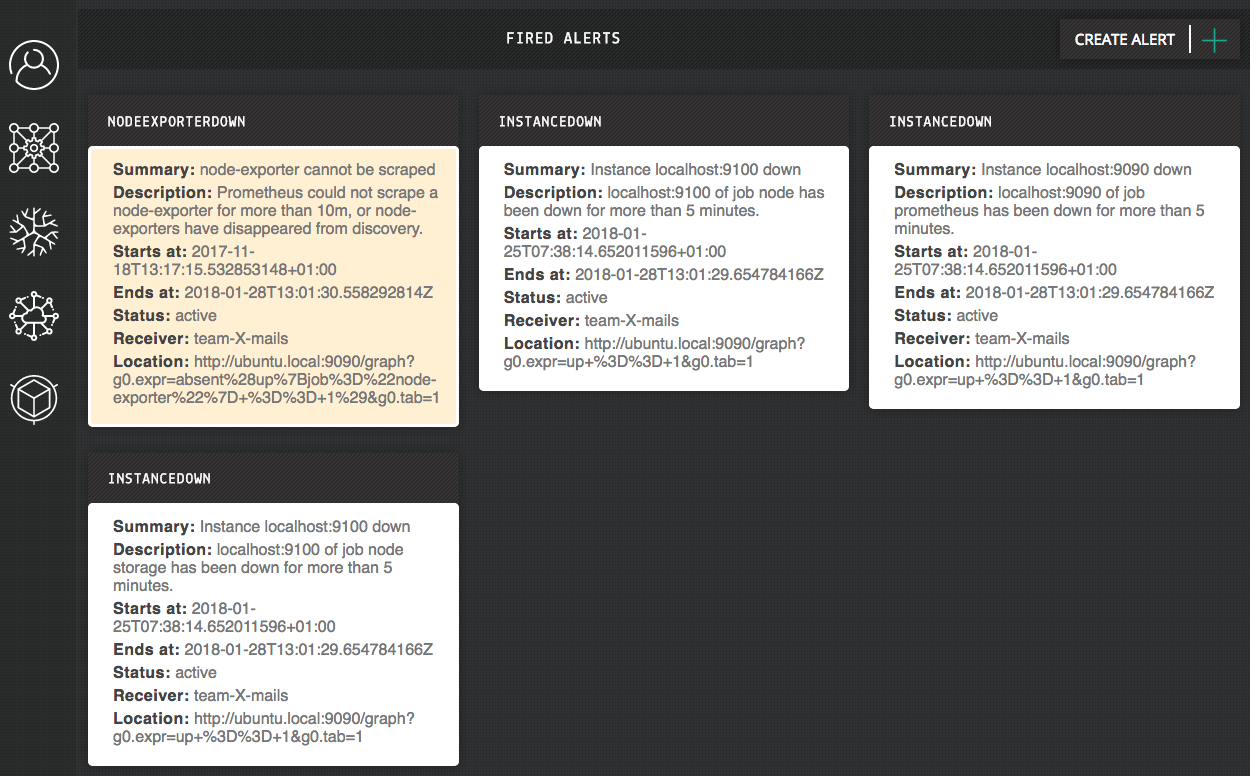
\includegraphics[width=\linewidth]{components/4/pics/alert_representation.png}
  \caption{N2Sky Administration Dashboard. Alerts representation}
  \label{fig:alert_representation}
\end{center}
\end{figure}

The view contains:

\begin{description}
\item[Header.] Header is the navigation bar with the title "Fired alerts" and the button. The button has the caption "Create Alert" and on click will initiate creating alert rule popup described in \autoref{Alerting rule creation} "Alerting rule creation".
\item[Alerts Grid] Contains three columns of alerts. When the alert end date is earlier than the current date, then this alert will not be shown. Only active alerts are visible. Detailed information about alert content is described in \autoref{Alerting Management System} "Alerting Management System".
\end{description}


